\begin{center}\large\textbf{Readings for Correlation and SLR: 11.1-11.5, 11.7-11.8}\\ %10.1-10.5 pg 378-420 and 10.7-10.8 pg 425-444 and 8.7 pg 305-311}\\
\normalsize \end{center}
\large ~\hrulefill
~\\
\textcolor{blue}{Until now, we've been considering a continuous variable (our response) and at least 1 categorical variable (our predictors) measured on the same individuals.  Now we'll investigate ways to analyze \textbf{two quantitative variables measured on the same units}.\\~\\
We'll start by looking at correlation and simple linear regression.  Later we'll move to multiple linear regression which has one response and $p$ quantitative predictors.  Finally, we'll combine the Multi-way ANOVA (factorial effects) modeling with this regression model in what are called \textbf{General Linear Models (GLMs)}.}\\~\\

\textbf{When is correlation appropriate?}\\
Consider having two variables $X$ and $Y$ (no need to designate one as a response and one as an explanatory).  We may want to look at the linear association between the two variables.\\~\\

That is, attempt to investigate how the two variables vary together.

\newpage

\textbf{Motivating example:} One type of fuel is biodiesel, which comes from plants.  An experiment was done to determine how much biodiesel could be generated from a certain type of plant grown in different media.  The final biomass was also recorded on 44 the plants from the experiment.  Let`s consider these two variables, the log of biodiesel and biomass.  \\

We can look at the distribution of each individually using our univariate descriptive methods (histogram, boxplot, mean/sd, etc.)\\
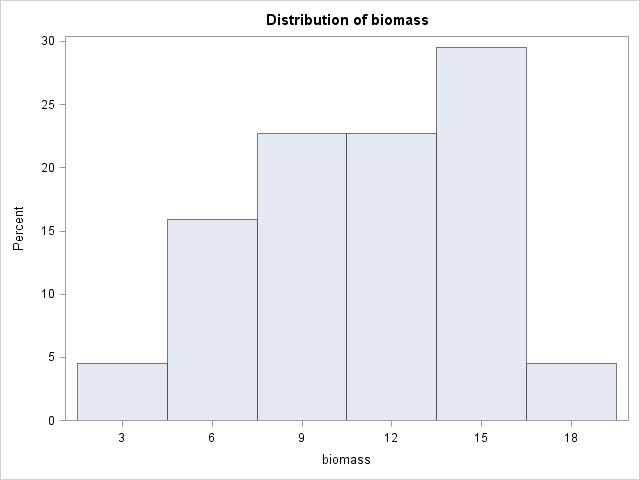
\includegraphics[scale=0.35]{biomasshist}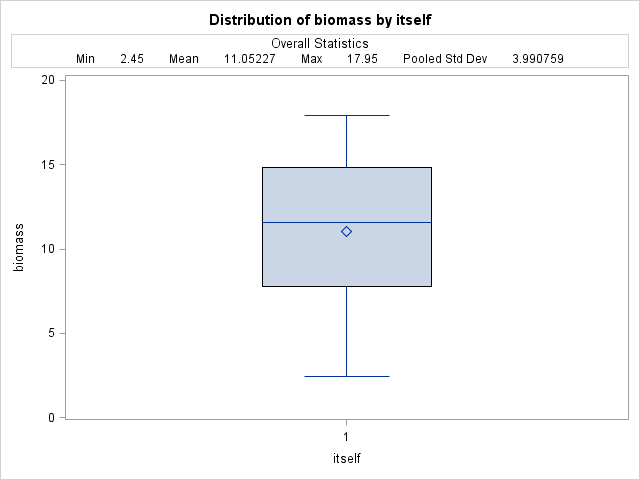
\includegraphics[scale=0.35]{biomassboxplot}\\
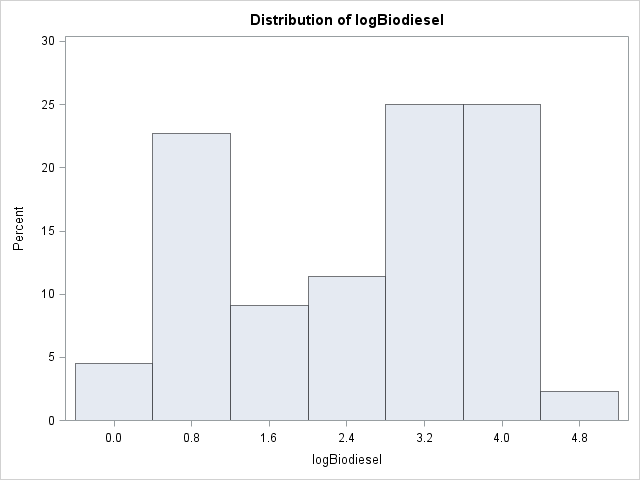
\includegraphics[scale=0.35]{logbiodieselhist}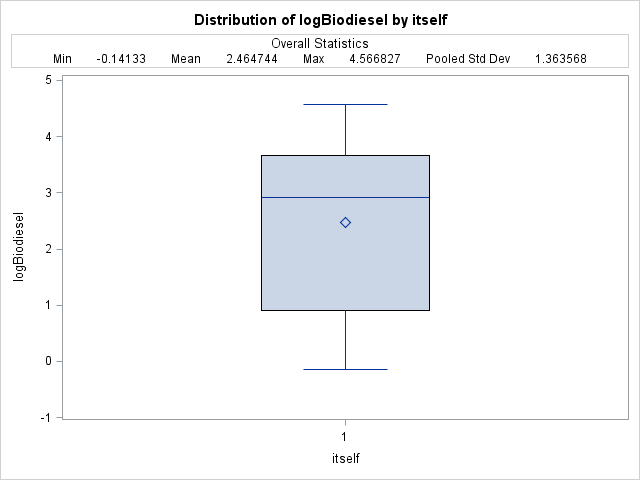
\includegraphics[scale=0.35]{logbiodieselboxplot}\\

How can we visually inspect the association between the two? A \textbf{Scatter plot} gives a visual approximation of the ``joint distribution'' between two variables.
\begin{center}
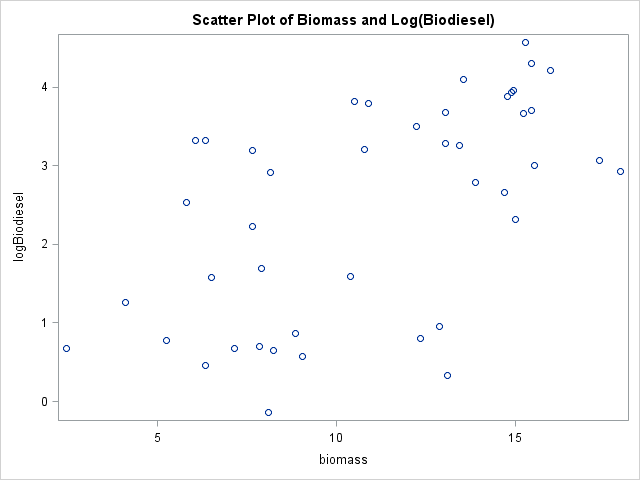
\includegraphics[scale=0.5]{scatterbiomasslogbiodiesel}
\end{center}

\newpage

What to look for in a scatterplot? \\
\begin{enumerate}
	\item \textcolor{red}{\textbf{Form}}
	%\underbar{~~~~~~~~~~~~~~~~~~~~~~~~~~~~~~~~~} 
	- Type of overall pattern: linear, quadratic, logarithmic etc.\\
	\item \textcolor{red}{\textbf{Strength}}
	%\underbar{~~~~~~~~~~~~~~~~~~~~~~~~~~~~~~~~~} 
	- Point closely or loosely follow the form?\\
	\item \textcolor{red}{\textbf{Direction}} 
	%\underbar{~~~~~~~~~~~~~~~~~~~~~~~~~~~~~~~~~} 
	- Pattern positive, negative, or NA?
\end{enumerate}

\begin{center}
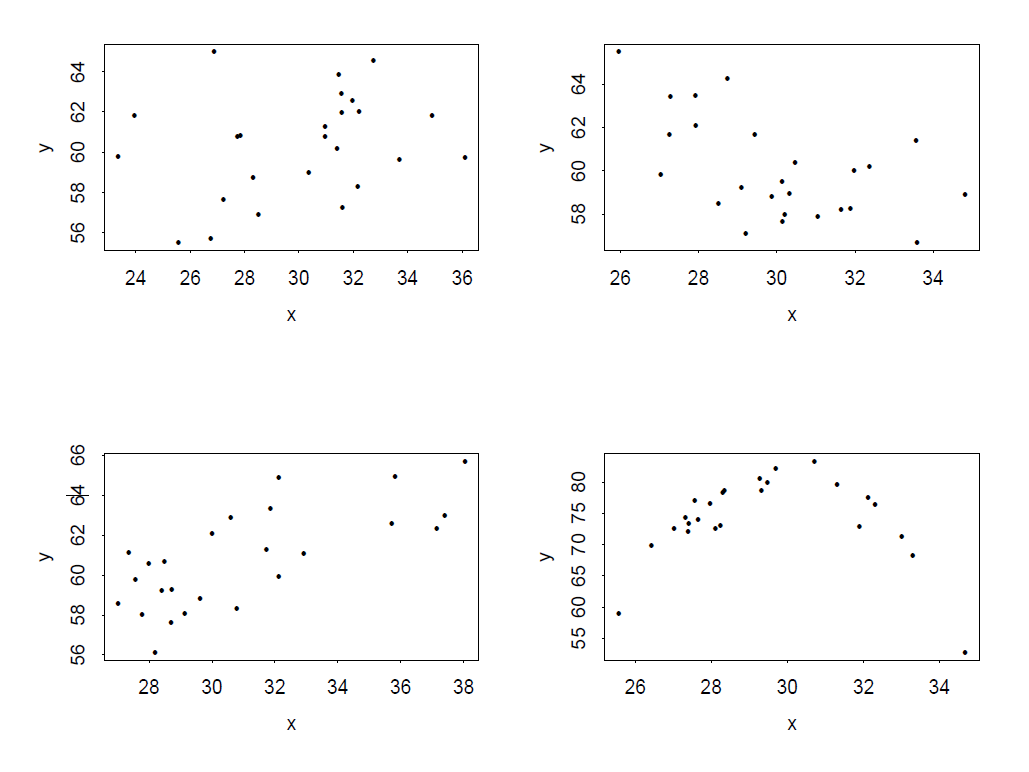
\includegraphics[height=3.5in,width=4.75in]{scattermatch}
\end{center}

\textit{\textcolor{blue}{With a histogram we might visually investigate the sample mean, which estimates a parameter of interest $\mu$.\\~\\
Similarly here, we can visually inspect the linear association, but there is also a statistic that measures this linear relationship.  \\~\\
We also have a parameter of interest here, which we label $\rho$ and call the correlation coefficient.}}

\newpage

\Large \textbf{The population correlation coefficient $\rho$.} \large\\~\\
\textbf{Correlation} is a unitless measure of the strength and direction of the \textit{linear} relationship between two RVs.\\~\\
$\rho$ or ($\rho_{_{XY}}$ when we want to be clear which variables we are talking about) is the population parameter that measures correlation between $X$ and $Y$.\\

The definition of $\rho_{_{XY}}$ is
$$\rho_{_{XY}} = E\left[\frac{(X-\mu_X)}{\sigma_X}\frac{(Y-\mu_Y))}{\sigma_Y}\right]=\rho.$$
Here, $E(\cdot)$ denotes mathematical expectation (basically meaning the average value of the function in the parenthesis).\\

This is similar to the way that the true mean of a random variable is defined, $\mu=E(Y)$ \\~\\~\\

\Large \textbf{The sample correlation coefficient $R$ and $r$.} \large\\~\\
Given $n$ independent pairs of quantitative data:
\begin{center}
\begin{tabular}{cc|c}
$ (x_1,y_1), (x_2,y_2), \ldots, (x_n,y_n) $ ~~~~~~~or~~~~~~~& Quant. Var 1 &	Quant. Var 2\\\cline{2-3}
&$y_1$	&$x_1$\\
&$y_2$	&$x_2$ \\
&$\ldots$&$\ldots$\\
&$y_n$ &$x_n$
\end{tabular}
\end{center}

\textbf{Sample correlation coefficient} - $r_{_{XY}}$ of the paired data is defined by 
$$ r_{_{XY}} = 
\frac{\frac{\sum_{i=1}^{n}(x_i - \bar{x})(y_i - \bar{y})}{(n-1)}}{\sqrt{\frac{\sum_{i=1}^{n}(x_i - \bar{x})^2}{(n-1)}*\frac{\sum_{i=1}^{n}(y_i -\bar{y})^2}{(n-1)}}} = \frac{s_{xy}}{s_x s_y}$$
$s_{xy}$ is called the sample covariance of $X$ and $Y$:
$$s_{xy}=\frac{\sum_{i=1}^{n}(x_i-\bar{x})(y_i-\bar{y})}{n-1}.$$
At times, this may be rewritten as 
$$ r_{_{XY}} = \frac{\sum_{i=1}^{n}(x_i - \bar{x})(y_i - \bar{y})}{\sqrt{\sum_{i=1}^{n}(x_i - \bar{x})^2*\sum_{i=1}^{n}(y_i -\bar{y})^2}}=\frac{S_{xy}}{\sqrt{S_{xx}S_{yy}}}$$

\newpage

Just as $\bar{Y}$ provides empirical information about a population mean $\mu_Y$, $R_{_{XY}}$ can be used for inference about the {\em population correlation coefficient} 
$\rho$.\\

\textcolor{blue}{Note, we can distinguish between the RV and the realized value, $R_{_{XY}}$ is an RV and $r_{_{XY}}$ is the observed value of that random variable}\\
	
\textbf{Properties of $r_{_{XY}}$}
\begin{itemize}
\item $r_{_{XY}}$ is an observed measure of the linear assn. between $X$ and $Y$ in a dataset.\\
\item correlation coefficient is unitless and always between -1 and 1:
$$ -1 \leq r_{_{XY}} \leq 1 $$~\\
\item The closer $r_{_{XY}}$ is to 1, the \textcolor{red}{stronger the positive linear association}\\
%\underbar{~~~~~~~~~~~~~~~~~~~~~~~~~~~~~~~~~~~~~~~~~~~~~~~~~~~~~~~~~~~~~~~~~~~~~~~~~~~~~~~~~~~~~~~~}\\
\item The closer $r_{_{XY}}$ is to -1, the \textcolor{red}{stronger the negative linear association}\\
%\underbar{~~~~~~~~~~~~~~~~~~~~~~~~~~~~~~~~~~~~~~~~~~~~~~~~~~~~~~~~~~~~~~~~~~~~~~~~~~~~~~~~~~~~~~~~}\\
\item The bigger $|r_{_{XY}}|$, the stronger the linear association \\
\item If $|r_{_{XY}}|=1$, then $X$ and $Y$ are said to be perfectly correlated (relationship is deterministic)\\
\item If $r_{_{XY}}\approx 0$, then no linear relationship.  Why?  (Note: We will do a test for $\rho=0$ later).
\end{itemize}
Some example scatter plots\\
\begin{flushleft}
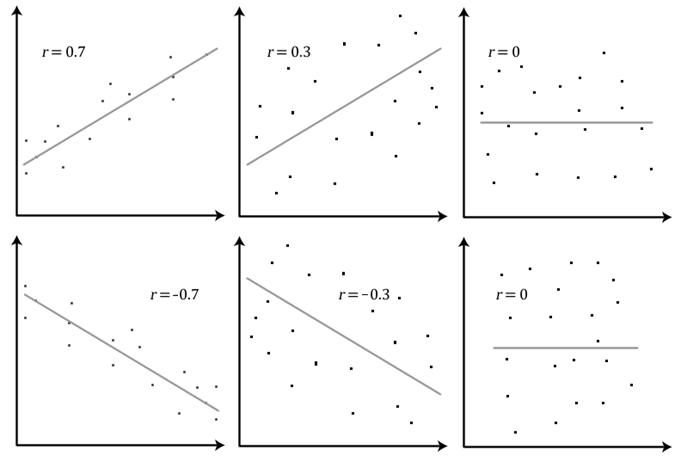
\includegraphics[scale=0.5]{scatterexamples}
\end{flushleft}
\newpage

For the log(Biodiesel) (call this $Y$) and Biomass (call this $X$) example we can compute the sample correlation coefficient using summary statistics: \label{bio}
$$ \bar{x}=11.0523, ~~~~ s_X=3.9908, ~~~~\bar{y}=2.4647, ~~~~ s_Y = 1.3636$$ 
$$ s_{_{XY}}=\frac{\sum_{i=1}^{n}(x_i-\bar{x})(y_i-\bar{y})}{n-1} = 3.1485$$
Applying the formula for $r_{_{XY}}$, we get
$$ r_{_{XY}}=\frac{s_{_{XY}}}{s_X s_Y}=\frac{3.1485}{3.9908 \times 1.3636} =0.5786$$~\\~\\~\\

Label the four plots below with the four sample correlation coefficients:
\begin{itemize}
\item $r=0.3$ ~~~~~~~~~~~~~~~~~~ $r=0.7$ 
\item $r=0.1$ ~~~~~~~~~~~~~~~~~~ $r=-0.6$ 
\end{itemize}
\begin{center}
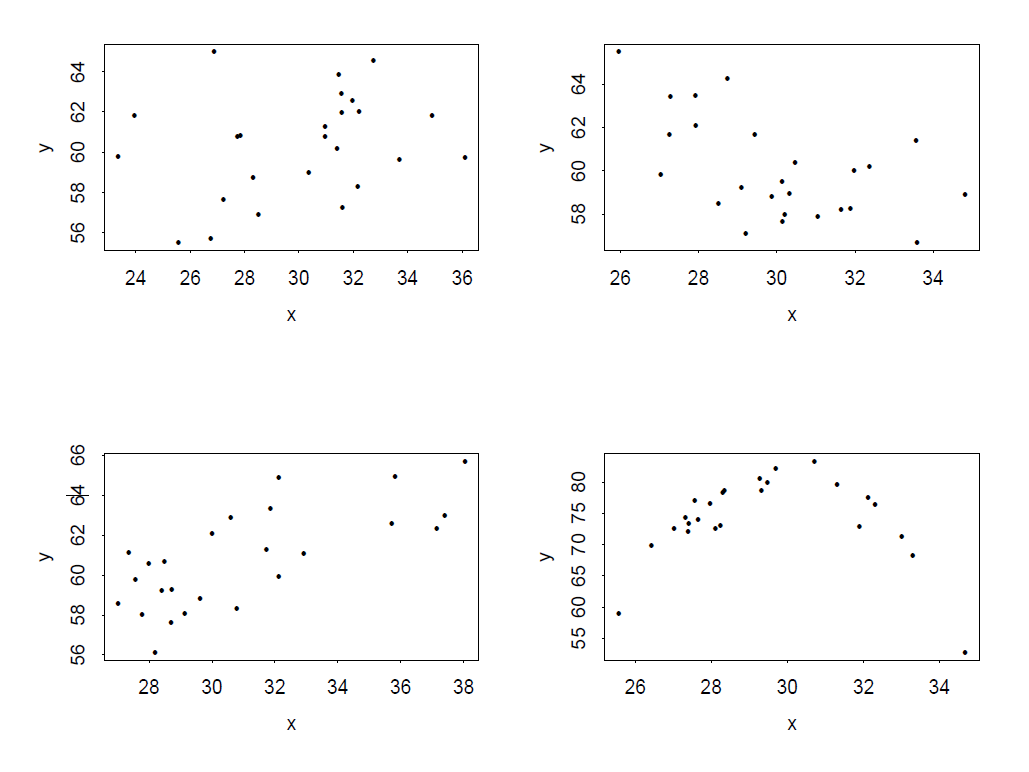
\includegraphics[height=3.5in,width=4.75in]{scattermatch}
\end{center}

\newpage

Would it be appropriate to use correlation to summarize the relationship between age and pace in the following scatter plot?  Why or why not?
\begin{center}
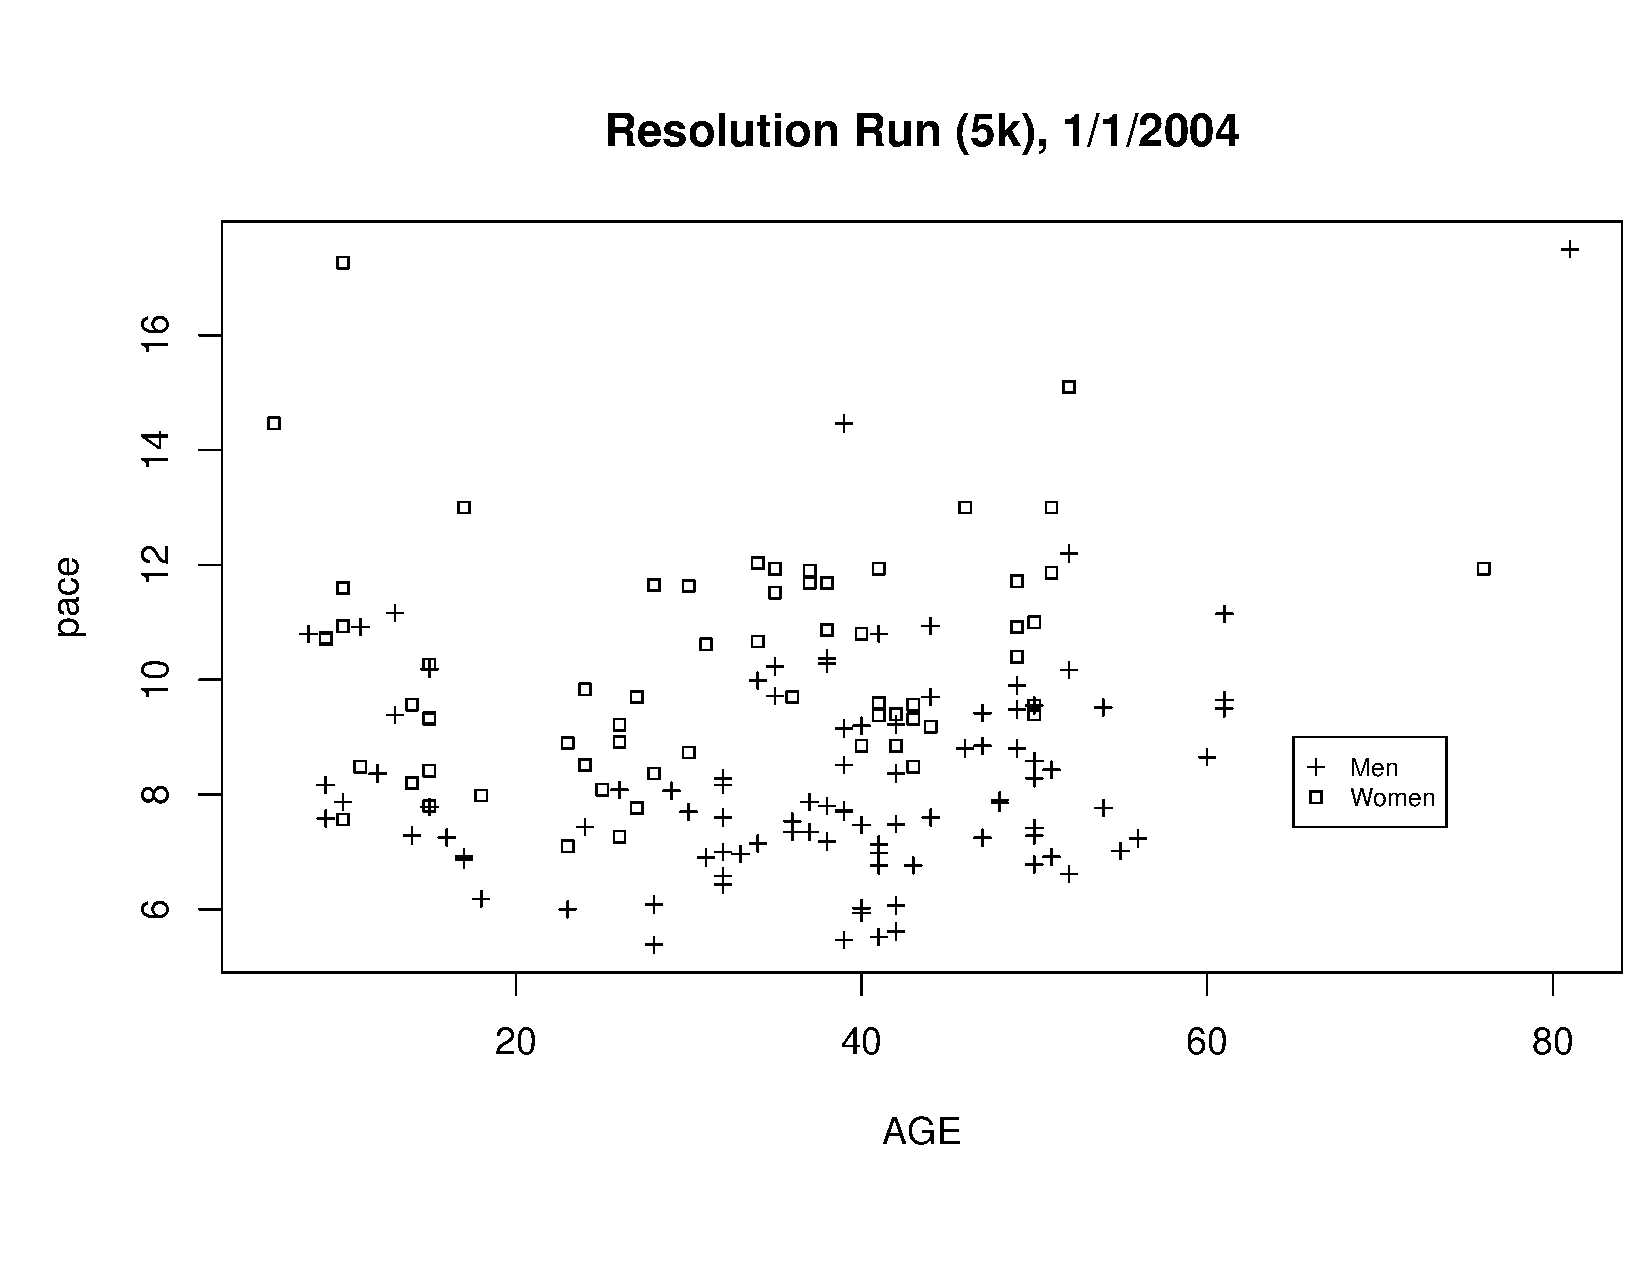
\includegraphics[scale=0.3]{res5k_nomodel.pdf}
\end{center}


\Large \textbf{Inference for $\rho$} \large\\

\textcolor{red}{\\$r$ is just a point estimate for $\rho$.  If we get a new sample, $r$ will change.  We want to use the sample value to make a claim about $\rho$.\\~\\
Relate to inference for $\mu$. $\bar{y}$ is a point estimate for $\mu$.  To make a claim or statement about $\mu$, we had to do a hypothesis test or a confidence interval.\\
This required knowledge of the \textbf{sampling distribution} of $\bar{Y}$ (or $\frac{\bar{Y}-\mu}{S/\sqrt{n}}$, a function of $\bar{Y}$).\\~\\
Similarly we need to know the distribution of $R$ or a function of $R$.}\\~\\

Much inference can somehow be related to the normal distribution.  
\begin{enumerate}
\item $R_{_{XY}}$ is between -1 and 1, so the normal distribution is not ideal for this statistic.
\item Instead we look at a transformation of $R$ that follows a normal distribution in `large' samples. Consider `Fisher's Transformation'
$$log\left(\frac{1+R}{1-R}\right)$$
\item When $R$ is very close to -1, we are approaching $log$ evaluated at 0.  When $R$ is very close to 1, we are approaching $log$ evaluated at $\infty$ - so it takes on values from $(-\infty, \infty)$. 
\item Thus, a test statistic useful for inference about $\rho$ is
$$Z(\rho)= \left(\frac{1}{2}\sqrt{n-3}\right)\left(\log \left(\frac{1+R}{1-R}\right) - \log \left(\frac{1+\rho}{1-\rho}\right)\right)\sim N(0,1)\mbox{ for large n}$$ 
\end{enumerate}

\newpage

\Large\textbf{To perform a Hypothesis Test about $\rho$:}\large\\
We often want to test the following hypotheses (although a one-sided test could be done),%\\~\\~\\~\\~\\~\\~\\
\textcolor{red}{$$H_0:\rho=0 ~~~~~~~~H_A: \rho\neq 0$$~\\~\\~\\~\\}

\textbf{Fisher's Z} - Assuming $H_0$ is true, the observed test statistic is 
$$z_{obs}=\left(\frac{1}{2}\sqrt{n-3}\right)\log\left(\frac{1+r}{1-r}\right)$$
The assumptions are that we have a large $n$ and a random $X$ and $Y$ (although if $X$ is fixed, inference still works ok).\\~\\
The reference distribution is the standard normal distribution.  \\~\\
%$$\mbox{Rejection Region: RR}=\left\{~~~~~~~~~~~~~~~~~~~~~~~~~~~~~~~~~~~~~~~~~~~~~~~~~~~~~~~~~~~~\right\}$$
\textcolor{red}{$$\mbox{Rejection Region: RR}=\left\{z_{obs}:|z_{obs}|>z_{\alpha/2}\right\}$$}
The p-value is found by %\\~\\~\\~\\
\textcolor{red}{$$2P(Z>|z_{obs}|)$$\\~\\~\\}
\textbf{T-test} - Assuming $H_0$ is true, another test statistic is
$$t_{obs}=\frac{r\sqrt{n-2}}{\sqrt{1-r^2}}$$
The assumptions are the $X$ and $Y$ have a `bivariate normal distribution' (although inference is robust to this assumption).\\~\\
The reference distribution is $t_{n-2}$.\\~\\
%$$\mbox{Rejection Region: RR}=\left\{~~~~~~~~~~~~~~~~~~~~~~~~~~~~~~~~~~~~~~~~~~~~~~~~~~~~~~~~~~~~\right\}$$
\textcolor{red}{$$\mbox{Rejection Region: RR}=\left\{t_{obs}:|t_{obs}|>t_{\alpha/2,n-2}\right\}$$}
The p-value is found by 
\textcolor{red}{$$2P(T_{n-2}>|t_{obs}|)$$}

\newpage

\textbf{For the log(Biodiesel) and Biomass example} our hypothesis test is:\\~\\
\textcolor{red}{
$$H_0:\rho=0 ~~~~~~~~H_A: \rho\neq 0$$~\\
Fisher's Z gives a test statistic of 
$$z_{obs}=\frac{1}{2}\sqrt{44-3}~log\left(\frac{1+0.5786}{1-0.5786}\right)=4.228$$
Using an $\alpha=0.05$ our rejection region is any $|z_{obs}|>1.96$.\\~\\
Our p-value $=2P(Z>4.228) = 2(0.00001) = 0.00002 < \alpha = 0.05$ so we reject our null hypothesis in favor of the alternative.  (Why do we multiply by 2?)\\~\\
What is the interpretation of the p-value=0.00002?  \\
The probability of getting a sample correlation (r) further (in magnitude) from 0 than 0.5786 assuming the true correlation ($\rho$) is 0 is 0.00002.\\~\\~\\
T-test gives a test statistic of 
$$t_{obs}=\frac{0.5786\sqrt{44-2}}{\sqrt{1-0.5786^2}}=4.597$$
Using an $\alpha=0.05$ our rejection region is any $|t_{obs}|>2.018$.\\~\\
Our p-value $=2P(T_{42}>4.597) = 2(0.00002) = 0.00004 < \alpha = 0.05$ so we reject our null hypothesis in favor of the alternative.
}

\newpage

\Large\textbf{To find a Confidence Interval for $\rho$:}\large\\
An approximate $100(1-\alpha)\%$ confidence interval for $\rho$ can be obtained by inverting the {Fisher transformation hypothesis test}:
$$ \left(\frac{\frac{1+r}{1-r}e^{-2z_{\alpha/2}/\sqrt{n-3}}-1}{\frac{1+r}{1-r}e^{-2z_{\alpha/2}/\sqrt{n-3}}+1}, \frac{\frac{1+r}{1-r}e^{2z_{\alpha/2}/\sqrt{n-3}}-1}{\frac{1+r}{1-r}e^{2z_{\alpha/2}/\sqrt{n-3}}+1}\right).$$
This formula differs slightly from that in the book, but it is equivalent.\\~\\~\\

Let's find a corresponding 95\% confidence interval for $\rho$ from the biodiesel and biomass example: \\~\\
$$\left(\frac{\frac{1+0.5786}{1-0.5786}e^{-2*1.96/\sqrt{44-3}}-1}{\frac{1+0.5786}{1-0.5786}e^{-2*1.96/\sqrt{44-3}}+1}, \frac{\frac{1+0.5786}{1-0.5786}e^{2*1.96/\sqrt{44-3}}-1}{\frac{1+0.5786}{1-0.5786}e^{2*1.96/\sqrt{44-3}}+1}\right) = (0.3401, 0.7471)$$~\\~\\
Interpret the interval in the context of the problem.  Also, state what confidence means here.
\textcolor{red}{\\~\\
We are 95\% confident that the true correlation ($\rho$) between log(biodiesel) and biomass is between 0.3401 and 0.7471.\\~\\~\\
When we say confident, we mean that if we did this experiment repeatedly (sample 44 plants, made measurements etc.) and made an interval for each experiment, the true correlation would fall in 95\% of the intervals created.}

\newpage

\textbf{How can we get SAS to do this for us?}
\begin{small}
\begin{verbatim}
proc corr data=bioexp FISHER(biasadj=NO) cov;
var biomass logbiodiesel;
run; 
\end{verbatim}
\end{small}
~\\~\\
\begin{center}
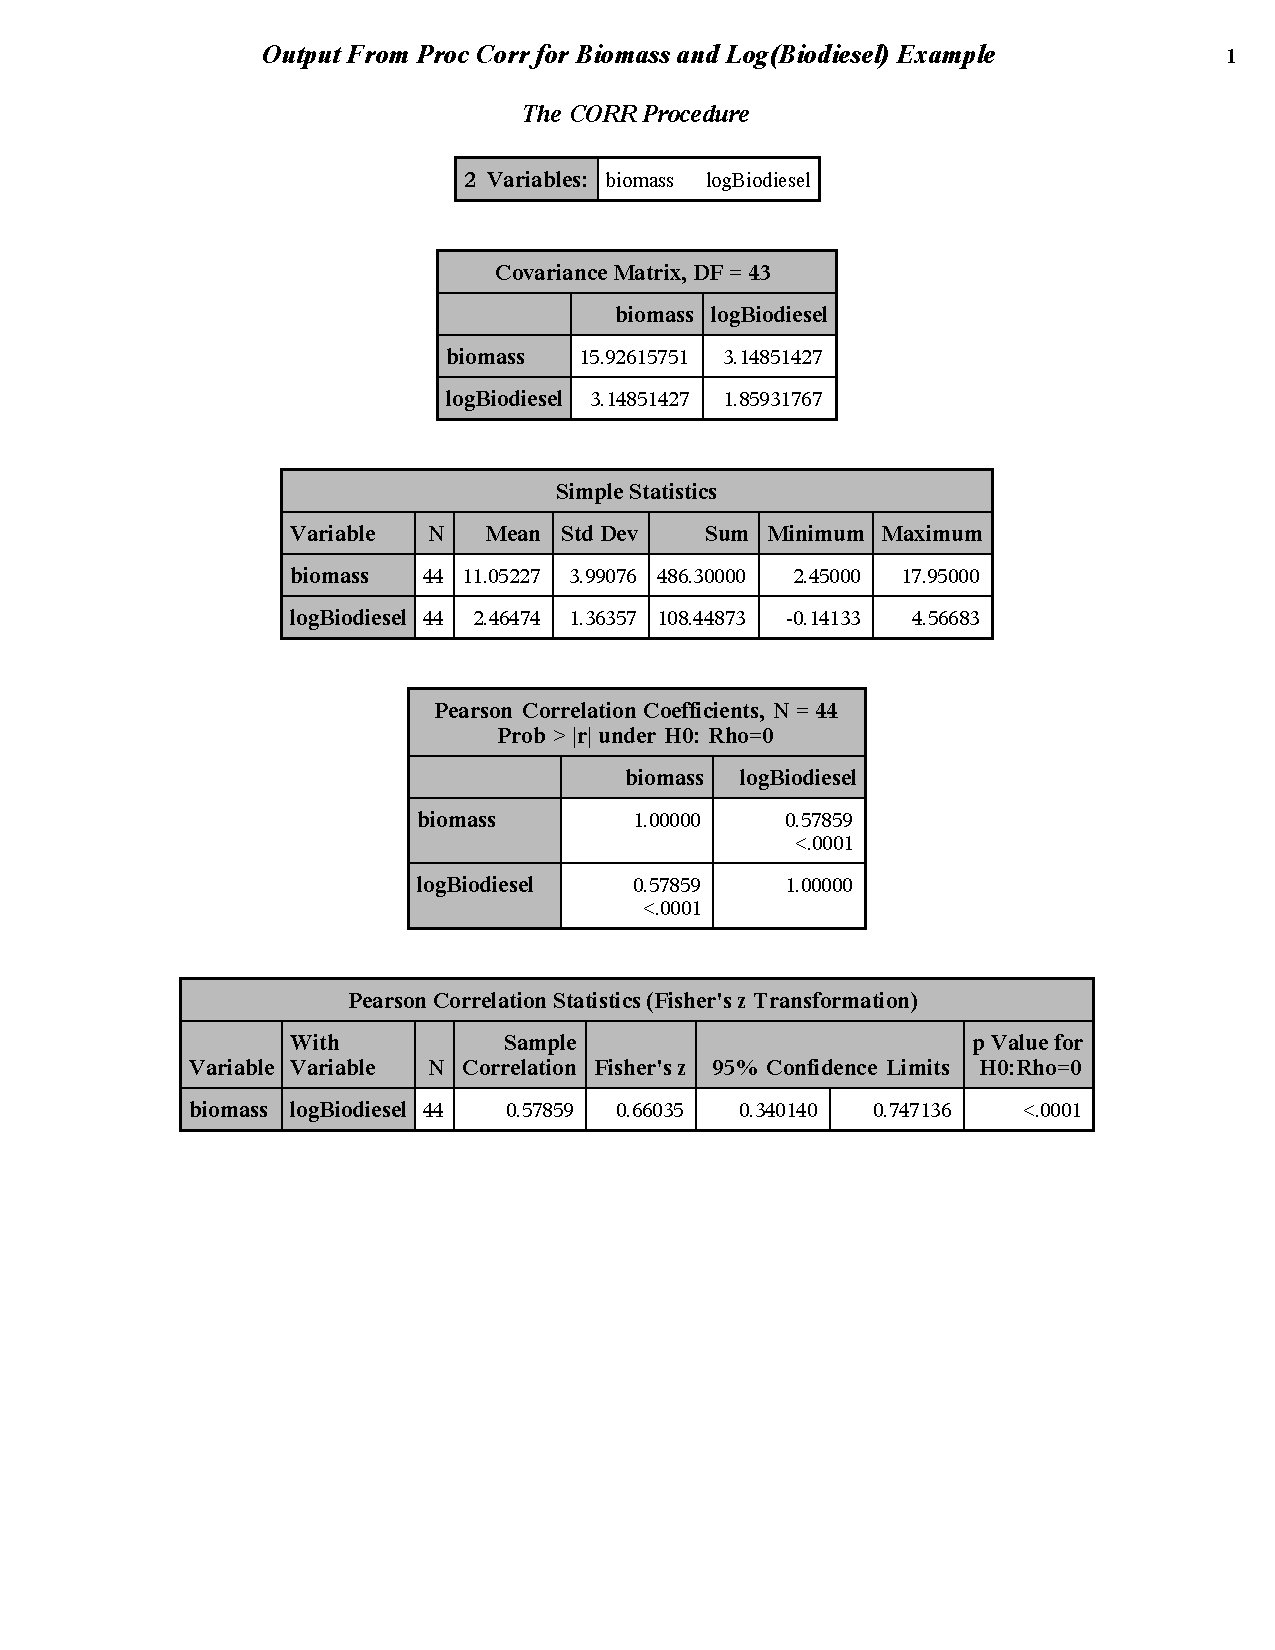
\includegraphics[scale=0.75,trim = 0mm 80mm 0mm 10mm]{corrbiodiesel.pdf}\label{corrbio}
\end{center}
~\\~\\
\textit{\textcolor{blue}{Note that there are also other statistics that measure the linear relationship.  The sample mean is strongly affected by outliers and so $r$ is as well.  Another version of correlation is Spearman's correlation.  This statistic uses the relative ranks of the data points rather than the values themselves.  This makes it more robust to outliers and a good statistic to use.}}

\newpage

\Large\textbf{Wrap up of Correlation}\large\\
When we have two quantitative variables, we want to describe the relationship between them.\\

A basic relationship is a linear one.  Correlation ($\rho$) is a statistical measure of this quantity.\\

We can estimate $\rho$ by $r$, the sample correlation.  A hypothesis test of interest is usually
$$H_0:\rho=0~~~~~~vs~~~~~H_A:\rho\neq0$$
The test can be carried out using a t-test or a normal based test.\\

Similarly a confidence interval can be created for $\rho$.\\

If the test is significant or the interval does not contain 0, then we know the two variables have a significant linear relationship. For instance, we may be able to conclude that having a high stress level is significantly associated with having high blood pressure.\\~\\~\\~\\~\\


\Large\textbf{Significant correlation does NOT imply causation!}\large\\
Please read the following famous examples of {\em spurious correlations}:
\begin{itemize}
\item A study finds a high positive correlation between coffee drinking and coronary heart disease.  Newspaper reports say the fragrant essence of the roasted beans of {\em Coffea arabica} are a menace to public health.
\item In a city, if you were to observe the amount of damage and the number of fire engines for enough recent fires, you would likely see a positive and significant correlation among these variables.  Obviously, it would be erroneous to conclude that fire engines cause damage.
\item {\em Lurking variable} - a third variable that is responsible for a correlation between two others.  (A.k.a. a possible confounding factor.)\\
An example would be to assess the association between say the reading skills of children and other measurements taken on them, such as shoesize.  There 
may be a statistically significant association between shoe size and reading skills, but that doesn't imply that one causes the other.  Rather, both are positively associated with a third variable, {\em age}.

\newpage

\item Among 50 countries examined in a dietary study, high positive correlation among fat intake and cancer (see figure, next page).  This example is taken from from {\em Statistics} by Freedman, Pisani and Purves.\\~\\
\begin{quotation} 
In countries where people eat lots of fat like the United States rates of breast cancer and colon cancer are high. This correlation is often used to argue that fat in the diet causes cancer. How good is the evidence?
\begin{center}
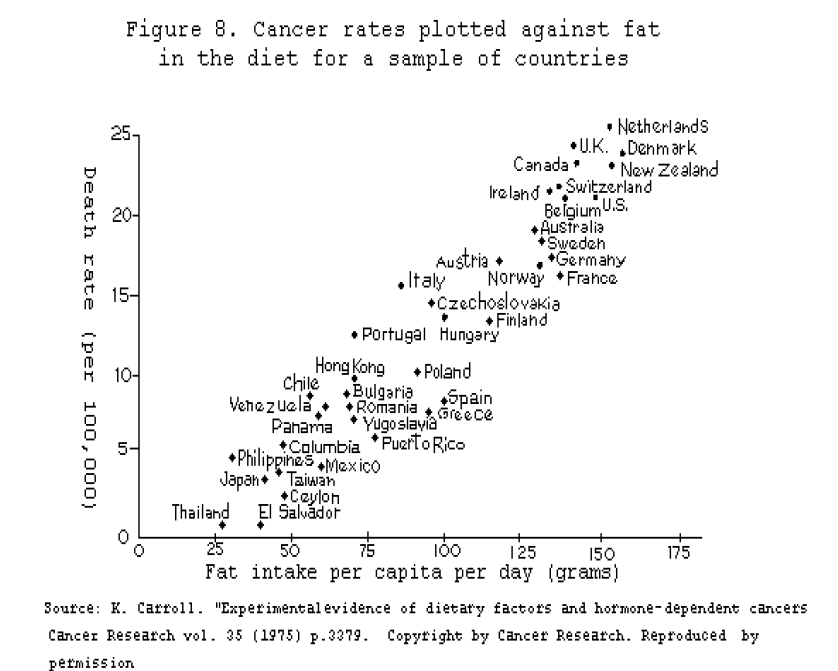
\includegraphics[scale=0.5]{scattercancer}
\end{center}
Discussion. If fat in the diet causes cancer, then the points in the diagram should slope up, other things being equal. So the diagram is some evidence for the theory. But the evidence is quite weak, because other things aren't equal. For example, the countries with lots of fat in the diet also have lots of sugar. A plot of colon cancer rates against sugar consumption would look just like figure 8, and nobody thinks that sugar causes colon cancer. As it turns out, fat and sugar are relatively expensive. In rich countries, people can afford to eat fat
and sugar rather than starchier grain products. Some aspects of the diet in these countries, or other factors in the life-style, probably do cause certain kinds of cancer and protect against other kinds. So far, epidemiologists can identify only a few of these factors with any real confidence. Fat is not among them. 
\end{quotation} 
(p. 152, {\em Statistics} by Friedman, Pisani, Purves and Adhikari)
\end{itemize}




%(Taken from {\em Statistics} by Friedman, Pisani, Purves and Adhikari.)
%%\newpage
%%A pertinent quotation from G. B. Shaw's {\em The Doctor's Dilemma:}
%%\begin{quotation}
%%Comparisons which are really comparisons between two social classes
%%with different standards of nutrition and education are palmed off as 
%%comparisons between the results of a certain medical treatment and its 
%%neglect.  Thus it is easy to prove the wearing of tall hats and the carrying of
%%umbrellas enlarges the chest, prolongs life, and confers comparative immunity
%%from disease; for the statistics show that the classes which use these articles are bigger, healthier, and live longer than the class which never dreams of 
%%possessing such things.  It does not take much perspicacity to see that what 
%%really makes this difference is not the tall hat and the umbrella, but the 
%%wealth and nourishment of which they are evidence \ldots
%%\end{quotation}
%\newpage
% ``torture the data until the true model confesses"





